\section{Near-Optimal layout}\label{near-optimal-layout}

Figure \ref{fig:near-optimal-layout} shows Near-optimal case. Here \glspl{access_point} are placed in the ground
so that both of them are in the center of the corresponding quarter (2nd and 3rd) 25x25 meters and far from all \glspl{ue} to approximately 25m.

\glspl{ue} located in two groups of three elements that fill the other two
quarters (1st and 4th) respectively.

At the same time, they keep a distance from each other to limit interference and hold the same conditions.

Finally, \gls{command_n_center} is set in the middle of whole 50x50 meters an
experimental field, so that 2 \gls{ap} and 2 groups of \glspl{ue} mentioned above are on the same distance.

\begin{figure}[H]
	\centering
	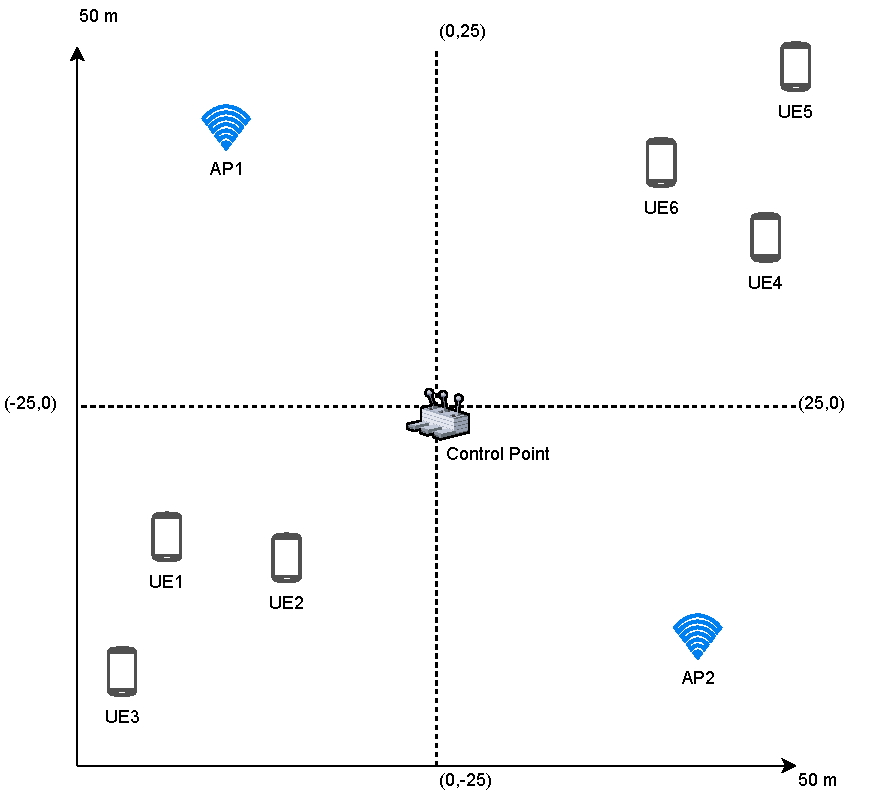
\includegraphics[width=0.7\linewidth,keepaspectratio]{images/05-cases-description-Near-Optimal.pdf}
	\caption{Near-Optimal layout}
	\label{fig:near-optimal-layout}
\end{figure}
